\clearpage
\section{DSP Laser Phase Noise Compensation}

\begin{tcolorbox}	
\begin{tabular}{p{2.75cm} p{0.2cm} p{10.5cm}} 	
\textbf{Student Name}  &:& Celestino Martins \\
\textbf{Goal}          &:& DSP algorithms for laser phase noise compensation applied in optical coherent receiver systems.\\
\textbf{Directory}              &:& sdf/dsp\_laser\_phase\_compensation
\end{tabular}
\end{tcolorbox}

The increasing digital traffic data demand in the core networks and the advances in digital signal processing (DSP) is pushing the deployment of coherent optical technology into optical networks. Based on this approach higher spectral efficient modulation formats can be used to increase the systems data rate, such as M-QAM. However, high order modulations are more susceptible to the different systems impairments such as chromatic dispersion (CD),
polarization mode dispersion (PMD), fibre nonlinearities and laser phase noise. Laser phase noise is one of the fundamental impairments in coherent optical systems, because it can severely limit the synchronization between transmitter and receiver in demodulation and detection of the transmitted data.
Since, in these modulation formats the data is encoded in the amplitude and phase of an optical carrier, an accurate carrier phase recovery is required.

In coherent optical systems, carrier phase recovery has been performed primarily in the electrical domain as part of the DSP, using both feedforward and feedback-based algorithms. Nevertheless, the researches experiments have shown that feedforward carrier phase recovery schemes are more tolerant to laser phase and facilitate the parallel implementation in a hardware unit, owing to the high parallelization and pipelining required in a real ASIC implementation. 

\subsection{Theoretical Analysis}
Generally, laser phase noise can be modeled as a Wiener process described as,
\begin{equation}
    \phi(k) = \phi(k-1)-\Delta \phi(k),
    \label{eq_phaseNoise}
\end{equation}
where, $\Delta \phi(k)$ is an independent and identically distributed random Gaussian variable with zero mean and variance given as,
\begin{equation}
    	\sigma^{2} = 2\pi(\Delta f T_\mathrm{s}),
    \label{eq_phaseNoise}
\end{equation}
where $\Delta f$ corresponds to the sum of linewidth of the signal and local oscillator lasers and $T_\mathrm{s}$ is the symbol period.

Typically, laser phase noise compensation for coherent optical receivers is performed by feedforward algorithms based on the well-known Viterbi-Viterbi (VV) algorithm or blind phase search algorithm (BPS). 
%These algorithms enable that a greater laser linewidth tolerance and facilitate the parallel implementation in a hardware unit.

\subsubsection{Viterbi-Viterbi algorithm}
\begin{figure}[h!]
    \centering
    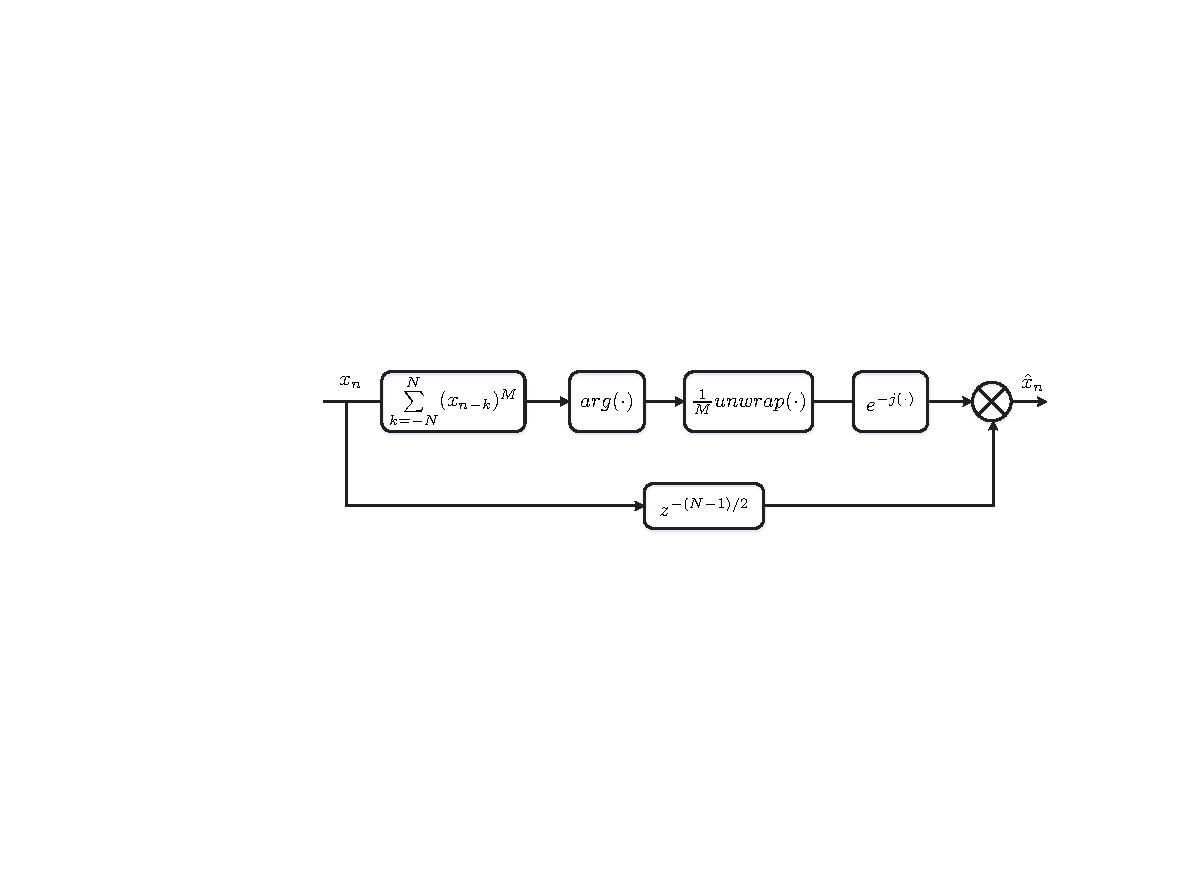
\includegraphics[width=\textwidth]{./sdf/dsp_laser_phase_compensation/figures/VV_phaseEstimation.pdf}
    \caption{Block diagram of Viterbi-Viterbi algorithm for carrier phase recovery.}
    \label{fig_VVdiagram}
\end{figure}
VV algorithm is a n-th power feed-forward approach employed for uniform angular distribution characteristic of m-PSK constellations, where the information of the modulated phase is removed by employing the n-th power operation on the received symbols. The algorithm implementation diagram is shown in Figure~\ref{fig_VVdiagram}, starting with M-th power operation on the received symbols. In order to minimize the impact of additive noise in the estimation process, a sum of $2N+1$ symbols is considered, which is then divided by M. The resulting estimated phase noise is then submitted to a phase unwrap function in order to avoid the occurrence of cycle slip. The final phase noise estimator is then used to compensate for the phase noise of the original symbol in the middle of the symbols block.


\subsubsection{Blind phase search algorithm}
\begin{figure}[h!]
    \centering
    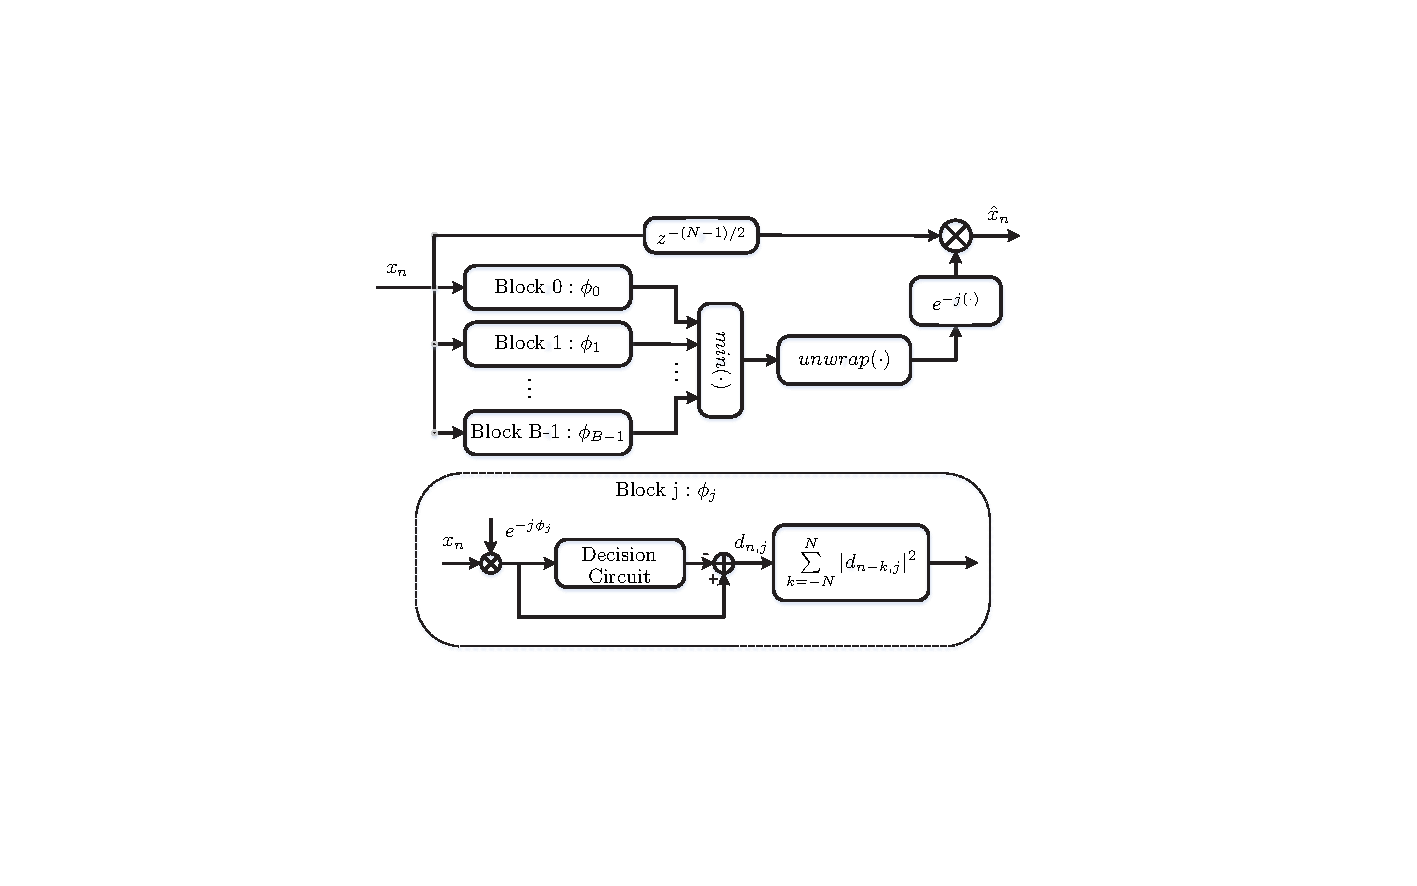
\includegraphics[width=12cm]{./sdf/dsp_laser_phase_compensation/figures/bps_diagram.pdf}
    \caption{Block diagram of blind phase search algorithm for carrier phase recovery.}
    \label{fig_BPSdiagram}
\end{figure}
An alternative to the VV phase noise estimator is the so-called BPS algorithm, in which the operation principle is shown in the Figure~\ref{fig_BPSdiagram}. Firstly, a block of $2N+1$ consecutive received symbols is rotated by a number of $B$ uniformly distributed test phases defined as,
\begin{equation}
    	\phi_{b} = \frac{b}{B}\frac{\pi}{2}, b \in\{0,1,...,B-1\}.
    \label{eq_phaseNoise}
\end{equation}
Then, the rotated blocks symbols are fed into decision circuit, where the square distance to the closest constellation points in the original constellation is calculated for each block. Each resulting square distances block is summed up to minimize the noise distortion. After average filtering, the test phase providing the minimum sum of distances is considered to be the phase noise estimator for the symbol in the middle of the block. The estimated phase noise is then unwrapped to reduce cycle slip occurrence, which is then used employed for the compensation for the phase noise of the original symbols.

\subsection{Simulation Analysis}

\subsection{Experimental Analysis}

\subsection{Comparative Analysis}



\bibliographystyle{unsrt}
%F. Munier, E. Alpman, T. Eriksson, A. Svensson, and H. Zirath, ``Estimation of phase noise for QPSK modulation over AWGN channels,'' in Proc. GigaHertz 2003 Symp., Linköping, Sweden, Nov. 4–5, 2003.
%
%T. Pfau, S. Hoffmann, and R. No\`{e}, ``Hardware-efficient coherent digital receiver concept with feed-forward carrier recovery for M-QAM constellations,'' J. Lightw. Technol., vol. 27, no. 8, pp. 989–999, Apr. 15, 2009.

\bibliography{bibliography} 